\section{Simulated samples}

The simulated (MC) samples are generated using Pythia 8. Some more blabla here ! \newline
In order to use our MC samples during the BDT training, described in Chapter \ref{sec:Selection}, and the calculation of efficiencies (Chapter \ref{sec: efficiency}), 
we have to make sure that the $\Bs\to\Ds\kaon\pion\pion$ decay is modelled correctly by the simulation. 
To check this we compare distributions of observables, which we use during the multivariate selection stage, as well as some key event observables. 
The compared distributions need to be generated by signal decays only, therefore we truth match all particles in the monte carlo samples. 
Signal distributions of observables in data are obtained using the sWeight technique \cite{Pivk:2004ty}: 
We perform a fit of a gaussian signal model and an exponential background to the invariant mass distribution of $\Bs\to\Ds\pion\pion\pion$ candidates (our normalization channel). 
Using the weights generated from this fit, we weight the distributions of data observables in $\Bs\to\Ds\kaon\pion\pion$ and obtain the corresponding signal distributions. \newline
Figure \ref{fig: MCbeforeWeighting} shows the distribution of the number of tracks per event and the distribution of the maximum ghost probability over all tracks, in MC and data.

\begin{figure}[h]
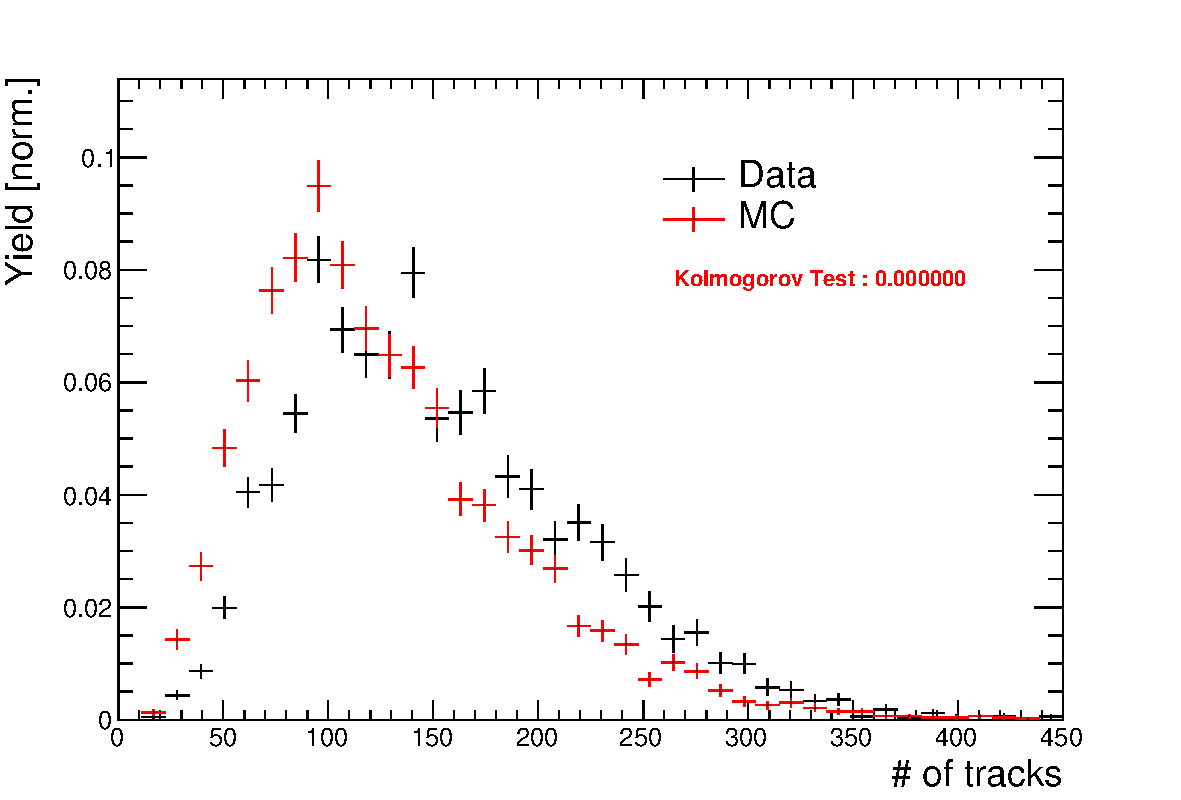
\includegraphics[height=6.cm,width=0.45\textwidth]{figs/nTracks.pdf}
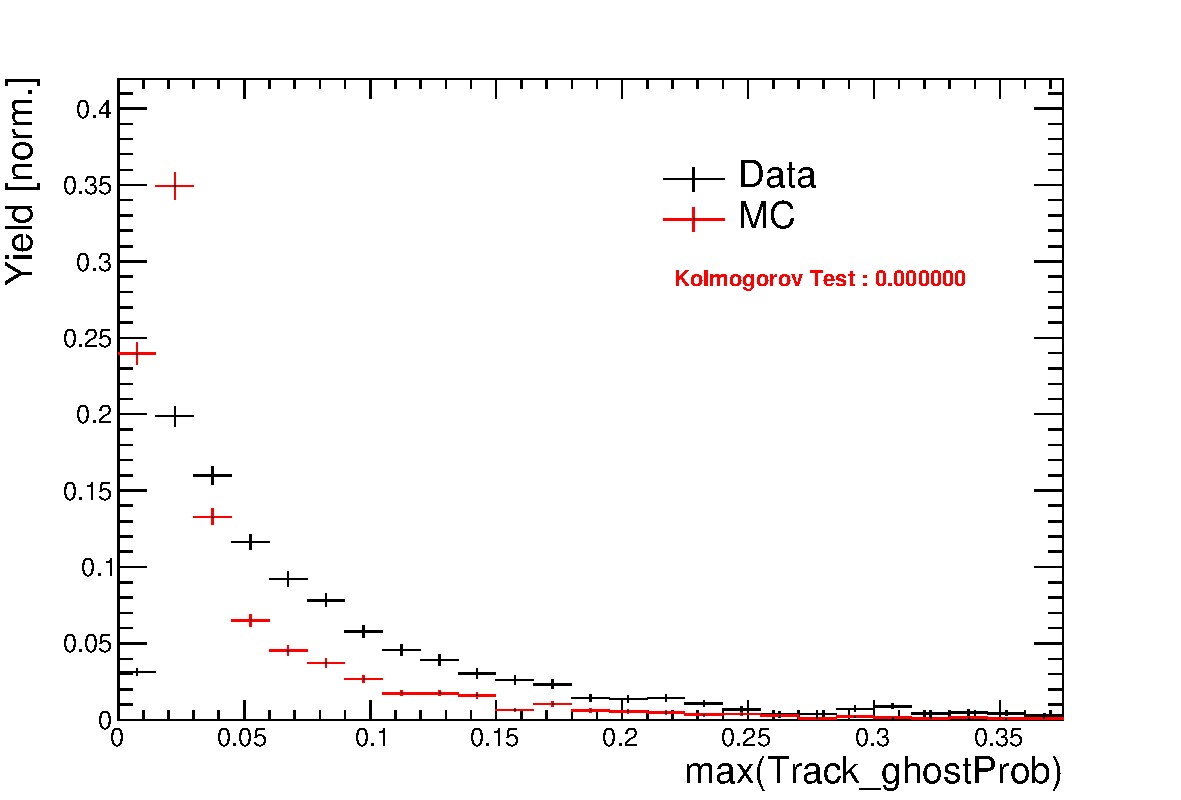
\includegraphics[height=6.cm,width=0.45\textwidth]{figs/max_ghostProb.pdf}
\caption{Comparison between the distribution of (left) the number of tracks and (right) the maximum ghost probability over all tracks, in (black) data and (red) simulation.}
\label{fig: MCbeforeWeighting}
\end{figure}


In both cases, the distributions differ significantly. Therefore, we re-weight the MC samples using those two variables. 
All distributions of observables used in the BDT training, before and after the re-weighting procedure, are shown in the Appendix \ref{sec: mcvdata}.                 
